\chapter{Literature}

\section{Psychological Foundations of Emotion in HRI}

\subsection{Essential Emotions for Human-Robot Interaction}

Emotions are fundamental to natural social communication, and social robots are increasingly designed with emotional intelligence so that they can ``infer and interpret human emotions'' during interaction. A widely adopted framework is Ekman's model of six basic emotions - happiness, surprise, fear, disgust, sadness, and anger - which are thought to have universal facial signals \cite{Reyes2019-go}. Later on Ekman's model of emotions was expanded at include a seventh basic emotion, contempt \cite{Matsumoto1992-jf}, though most omit this. Empirical HRI systems typically choose a subset of basic emotions that are most relevant and reliably detectable. For example, Alonso-Martín et al.\ \cite{Alonso-Martin2013-cv} deliberately limited their NAO-based system to neutral, happiness, sadness, and surprise, noting that these four cover the key dialog cases and are easier to recognise by camera and microphone.

It is essential for HRI systems to detect and respond appropriately to happiness. Smiling or laughter from a user typically means things are going well, and robots that recognise happiness can respond by building rapport. In practice, happy expressions are readily recognised by current systems: for instance, a NAO robot using a CNN achieved approximately 91\% accuracy on happy faces \cite{Filippini2021-ni}.

Sadness usually signals that something is wrong. Robots that recognise sadness can respond empathetically (e.g.\ speaking softly or offering help). Many HRI experiments explicitly use sadness as a target emotion \cite{Stock-Homburg2022-wd}. Detection systems also handle sadness well, for example, the same NAO running a CNN as above, recognised sad faces with approximately 90\% accuracy \cite{Filippini2021-ni}. Sadness is a core negative state for social robots to sense; it is included in nearly every emotion set, and responding to it (e.g.\ consolation) supports natural interaction.

Anger detection is critical for managing conflict or danger. An angry expression can indicate frustration, disagreement, or risk. Anger is a high-arousal signal of dissatisfaction \cite{Stock-Homburg2022-wd}. Practically, if a robot detects that a person is angry, it can take steps to defuse the situation (apologise or give space). Recognition of anger tends to be good (85\% accuracy in one study \cite{Ramis2020-ec}). Since anger often requires adjustment of robot behavior, it's widely treated as an essential emotion in HRI \cite{Stock-Homburg2022-wd}.

HRI systems also consider fear and surprise important, but usually to avoid. Inducing fear or startling people is known to harm trust. In HRI safety research, for instance, Sisbot et al.\ \cite{Sisbot2010-wy} emphasise that a socially acceptable robot must never trigger human fear, surprise or discomfort. Thus, some HRI systems include fear/surprise detection mainly to monitor safety (e.g.\ pausing if a user appears startled), though it is sometimes harder to detect (about 65\% accuracy in the NAO study \cite{Filippini2021-ni}).

Disgust is the least-studied of the six in social robotics, but it is included for completeness. In human social signaling, disgust usually means ``this is aversive'' (e.g.\ a bad smell or morally repugnant content). Few HRI applications explicitly focus on disgust, but it is part of standard emotion sets \cite{Stock-Homburg2022-wd}. When detected, a robot might interpret disgust similarly to anger/avoidance (e.g. stop a disagreeable action). Recognition of disgust tends to be lower (it was grouped with sadness and fear at approximately 65\% accuracy \cite{Filippini2021-ni}). Thus, while disgust is acknowledged as a basic human emotion, most HRI systems prioritise the others; it is included mainly to round out the universal facial expression categories.

A ``neutral'' state is normally treated as another category. Most human interaction is emotionally neutral, thus systems include it as a catch-all \cite{Alonso-Martin2013-cv}.

Finally, contempt is rarely a focus in HRI systems. Most HRI emotion-recognition work uses Ekman's orignial basic categories (anger, disgust, fear, happiness, sadness, surprise, and a neutral catagory) and often omits contempt. Some commercial APIs (e.g. Microsoft's Face API) do output contempt, but empirical HRI studies find almost no contemptful expressions in practice \cite{Chuah2021-zw}. In short, contempt is technically included in some classifiers, but it's not commonly reported or reliably detected in real HRI data.

Overall, recent HRI research converges on Ekman's six basic emotions as the ``core'' set that robots should recognise, most commonly ommiting the seventh emotion, contempt. Happiness and surprise are seen as especially beneficial for positive user experience, whereas anger, sadness, and fear are included so robots can handle conflict or distress appropriately \cite{Chuah2021-zw}. Disgust is rarely targeted. Overall, the ``essential emotions'' for effective HRI turn out to be those that (a) humans naturally express strongly in social settings and (b) robots can reliably sense the core Ekman emotions plus a neutral baseline.

\subsection{Appraisal Theory}

Appraisal theory accounts for the elicitation of emotion by linking it to an individual's cognitive evaluation of events, particularly in terms of goal relevance, perceived control, certainty, and agency. Thus it explains why identical events may evoke divergent emotional responses across individuals \cite{Suhaila_2021-ez}. This theoretical perspective has informed several computational approaches to emotion modeling. For instance, knowledge-based systems such as EmotiNet represent prototypical event-action sequences and their associated affective outcomes based on predefined appraisal rules \cite{Balahur2011-mb}. In the domain of emotion analysis, appraisals have been used as intermediate representations to support more interpretable and robust classification. Troiano et al.\ \cite{Troiano2023-if} introduced a corpus comprising event descriptions annotated with both emotion labels and appraisal dimensions, demonstrating that appraisal features can be automatically inferred from text with near-human reliability. Critically, they showed that incorporating appraisal representations alongside emotion categories enhanced classification accuracy, suggesting that appraisal-based reasoning provides a complementary pathway for modeling affective meaning, particularly in cases involving implicit cues, such as goal obstruction leading to anger or fear.

Within affective HRI, appraisal-informed models enable artificial agents to infer users' emotional states by assessing interaction context, such as whether the agent's actions support or hinder user goals. Some implementations explicitly encode appraisal variables (e.g., task success, goal congruence, user feedback) alongside perceptual cues. Demutti et al.\ \cite{Demutti2022-vz}, for example, proposed a cloud-based HRI framework wherein user-reported appraisals (e.g., satisfaction with conversational topics and task outcomes) were integrated with facial and gaze data. A Random Forest classifier trained on both appraisal and sensory features outperformed models relying solely on perceptual input when classifying affective valence.

In broader HRI contexts, appraisal theory has been leveraged to imbue robots with more human-like emotion reasoning capabilities. For example, Tang et al.\ \cite{Tang2025-ny} describe an architecture wherein robots continuously evaluate the valence, relevance, and goal impact of human behaviors in real time. Drawing on models such as the Ortony, Clore, and Collins (OCC) framework, the robot applies appraisal rules to determine whether events are congruent with user goals and generates contextually appropriate affective responses. In experimental scenarios, appraisal-enabled robots demonstrated improved social responsiveness; for instance, one robot correctly interpreted a student's disappointment, despite incongruent verbal cues, and provided empathetic feedback, whereas a non-appraisal baseline failed to recognise the underlying emotion and responded inappropriately.

\subsection{Valence-Arousal model}

Alongside cognitive appraisal, many emotion-aware systems use dimensional models of affect, which map emotions onto continuous scales. The most common framework is the valence-arousal (VA) space (often called Russells circumplex model \cite{Russell1980-cd}). In this model, valence corresponds to pleasantness (positive vs.\ negative affect), while arousal corresponds to activation or intensity (calm vs.\ excited). Every emotional state can be placed as a point in this 2D space: for example,``joy'' is high-valence, high-arousal, while ``sadness'' is low-valence, low-arousal. These two dimensions capture the core affective quality of most emotions \cite{Marmpena2018-tw}.

\begin{figure}[!htb]
    \centering{}
    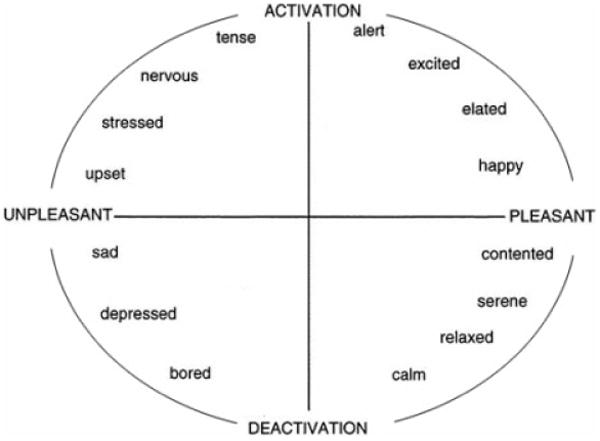
\includegraphics[scale=0.80]{lit_review_images/RussellsCircumplex.jpg}
    \caption{A Graphical representation of Russell's Circumplex Model of Affect \cite{Russell1980-cd}.}
    \label{fig:RussellsCircumplex}
\end{figure}

Dimensional labeling is popular in HRI because it provides a common language across modalities and datasets. For instance, researchers often annotate facial expression or physiological data with valence-arousal values so that different sensors can be merged or compared. In fact, Spezialetti et al.\ \cite{Spezialetti2020-ty} note that ``several dimensional annotated datasets share a common valence-arousal (VA) representation, which allows comparing and merging data from different datasets''. As a result, VA labels are often provided as a good practice in emotion datasets. By covering a broad range of VA values, such datasets enable training models that predict continuous affect.

In affective computing systems (vision, speech, multimodal recognition), VA is also apparent. Modern facial emotion recognition benchmarks (like the ABAW challenge) include frame-by-frame valence/arousal estimation as official tasks. Multi-task deep models extract features from faces (e.g.\ with EfficientNet) and output both discrete expression labels and continuous VA scores \cite{Savchenko2024-ns}. These continuous predictions allow systems to gauge nuanced changes in affect (e.g.\ gradual smiles) rather than hard categories. Similarly, speech-based emotion models often regress valence and arousal from audio features.

\section{Facial Emotion Recognition}

Facial emotion recognition is a crucial aspect of affective computing \cite{Picard2000-mt} that involves analysing facial expressions to identify human emotions. This skill is essential for successful interactions between people and is particularly important in the realm of HRI. For robots to respond to human emotions promptly, facial emotion recognition is key. When aware of human emotions, robots can interact more naturally with humans by quickly and accurately recognising emotions. More natural interaction capability will favour acceptance and use of robots in peoples lives.

\subsection{Datasets}

Pierre Luc Carrier and Aaron Courville \cite{Goodfellow2013-al} introduced the Facial Expression Recognition 2013 (FER-2013) dataset as part of a larger project aimed at advancing emotion recognition research. Created using the Google image search API, it collected images matching 184 emotion-related keywords like `blissful' and `enraged.' The dataset includes nearly 36,000 images, processed using OpenCV for face detection and manually curated for accuracy. These images were resized to 48\(\times\)48 pixels, converted to grayscale, and categorised into seven broad emotion classes: Anger, Disgust, Fear, Happiness, Sadness, Surprise, and Neutral.  It serves as a crucial resource for training and evaluating emotion recognition models, being the most used data set for review of articles.

AffectNet \cite{Mollahosseini2017-bj} is a large-scale facial expression dataset introduced to address the need for more diverse and comprehensive data in facial emotion recognition. It contains over one million images of faces collected using emotion-related keywords translated into multiple languages on three different search engines (Google, Bing and Yahoo). These images were manually annotated into eight different emotion categories: neutral, happy, sad, surprise, fear, disgust, anger, and contempt, along with additional labels for valence and arousal. AffectNet stands out due to its extensive size, diversity in ethnicity, age, and conditions such as pose and lighting variations, making it a valuable resource for training and evaluating emotion recognition systems.

JAFFE \cite{jaffe}  and CK+ are both smaller, highly curated datasets. JAFFE contains 213 images of posed facial expressions from 10 Japanese female models, labelled with six basic emotions plus neutral. It is often used for cross-cultural studies of emotion recognition. CK+, meanwhile, includes 593 video sequences from 123 subjects, with each sequence showing a transition from a neutral face to a peak expression. CK+ is notable for including both emotion and action unit labels, providing fine-grained information about facial muscle movements, making it a strong choice for both emotion and FACS-based studies. KDEF \cite{Lundqvist2015-in}, a separate dataset of 4,900 images from 70 individuals, focuses on a broader demographic range and is often used for validation in emotion recognition systems.

\subsection{Algorithms}

Convolutional Neural Networks (CNNs) have emerged as the dominant approach in the realm of vision-based emotion recognition for robotic systems. Researchers typically adopt a two-phase methodology, first using CNNs for the extraction of features, followed by the implementation of classification techniques. One study introduces a multistep technique that aims to improve facial recognition accuracy. It begins with the application of a histogram equation to enhance image contrast, which is then succeeded by a bilateral filter to reduce noise while maintaining edge integrity. Then, the Viola-Jones (Haar-Cascade) face detection algorithm in OpenCV is utilised to pinpoint the facial area within the input image. The proposed technique further refines the extraction of features through an innovative variant of local binary pattern (LBP), which takes advantage of a convolution filter and a Kirsch operator to capture features that withstand variations in illumination, scaling, and rotation \cite{Mistry2020-gr}.

\begin{figure}[!htb]
    \centering{}
    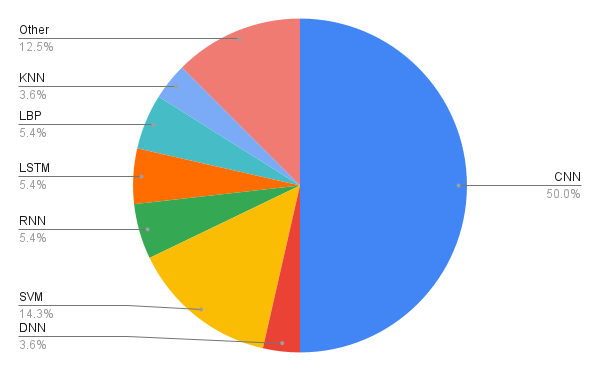
\includegraphics[scale=0.50]{lit_review_images/chartFaceModelUsage.png}
    \caption{A summary of the algorithmic choices used in the reviewed studies.}
    \label{figure:alorithmUsage}
\end{figure}

Figure \ref{figure:alorithmUsage} summarises the underlying network types used in all reviewed studies, showing the prevalence of CNN-based methods and the relative frequency of other algorithmic choices.

Facial expression analysis remains one of the most practical non-invasive modalities for emotion recognition in HRI. However, most systems rely on outdated or limited face detection methods like using Haar-Cascade for initial face detection and cropping the image to isolate the face before implementing more advanced CNNs \cite{Appuhamy2018-dc} or SVMs \cite{Gupta2018-af} \cite{Rosula_Reyes2020-yz}, show promise for working in resource-limited environments. One study used a Haar cascade to quickly locate faces, followed by a CNN to extract features, and finally a long-short-term memory network \cite{8760246} to perform classification. Other studies have used a convolutional autoencoder and support vector regressors \cite{Allognon2020-um} or recurring neural networks \cite{Brandizzi2021AutomaticRI} to incorporate temporal features into emotion recognition and establish correlations between facial expression transformations and the six basic emotions.

In a study by Kusuma et al.\ \cite{Kusuma2020-oa}, VGG16 was effectively used for emotion recognition on the FER dataset. Their model achieved an overall accuracy of 69.4\% after careful optimisations through specific configurations, such as using an imbalanced dataset (they did not use data augmentation to rectify the heavy imbalances within the dataset), Global Average Pooling (GAP), non-frozen layers, and the Stochastic Gradient Descent (SGD) optimiser. This model has potential for real-time applications in HRI.

ResNet50 was used to a high degree of accuracy on FER-2013 by Pramerdorfer et al. \cite{Pramerdorfer2016-xx}, achieving 72.4\% accuracy with 5.3 million trainable parameters. No special modifications were made to the network, except removing the initial convolution and pooling layer and narrowing the architecture by using 256 feature maps in the final residual group, thereby reducing the parameter count. While the model remains relatively large by embedded deployment standards, its high reported accuracy makes it a strong candidate for emotion recognition in HRI. However, its real-world feasibility depends on whether its inference speed and computational demands can be tolerated on resource-constrained robotic platforms.

Shenoy et al.\ \cite{9900581} presents the design of an adaptive learning system for real-time emotion recognition in humanoid robots. The system continuously updates individualised models based on user interactions, improving performance over time. It employs an ensemble of ResNet50 and Inception v3 networks, leveraging transfer learning to enhance emotion recognition from facial expressions. They performed a two-stage user study featuring 75 participants using the results for stage one to personalise the experience in stage two. The robot's adaptive actions used the recognised emotions to engage users in social interactions and to elicit emotional responses, such as trust, empathy, and engagement. Results showed a 12\% improvement in emotion recognition accuracy and an 8.28\% increase in the success rate of emotion elicitation between stages, showcasing the system's ability to adapt and foster meaningful social interactions.

I-MobileNetV2, an enhanced version of MobileNetV2 proposed by Zhu et al.\ \cite{Zhu2024-gy}, aimed to improve facial emotion recognition tasks by addressing issues such as large parameter quantities, loss of feature information and low accuracy rates. Key modifications include the retention of depthwise separated convolution for computational efficiency, a reverse fusion mechanism to preserve negative features, the use of the SELU activation function to avoid gradient vanishing, and the integration of the SE-Net channel attention mechanism to improve feature recognition. These enhancements resulted in recognition accuracies of 68.62\% on FER2013 and 95.96\% on CK+, with an 83.8\% reduction in parameter count.

Despite these improvements, the accuracy gains over the base MobileNetV2 are modest, with only a 0.72\% increase on FER2013 and 6.14\% on CK+. However, the reduction in parameters should significantly improve inference speeds over the MobileNetV2 base model. However, MobileNetV2 alone shows good performance on FER2013, achieving 67.9\% accuracy with 2.2 million parameters, making it a strong candidate for real-time applications in HRI.

Data augmentations have been employed in various approaches to enhance facial emotion recognition, often in conjunction with conventional CNNs. Several studies have demonstrated that augmenting training data can improve model performance by addressing challenges such as class imbalances and overfitting \cite{Saxena2022-sr} \cite{Ruiz-Garcia2018-uy}. A particularly successful technique involved Generative Adversarial Networks (GANs) for data augmentation, as demonstrated by Song and Kwon (2019). Their study also emphasised the importance of including the lower half of the face during training to improve the accuracy in detecting emotions through facial recognition.

\subsection{Applications}

The exploration of applications is also apparent, ranging from studies investigating and improving the effectiveness of emotion recognition in older adults \cite{Ma2019-ng} to those focusing on unconstrained environments \cite{Webb2020-bq} and those with the goal of creating a robot capable of helping speech therapy through the ability to articulate words similar to that of human speech \cite{Esfandbod2023-eq}, through the development of facial expression recognition and lip syncing capabilities, the RASA robot aims to engage children and enhance their learning outcomes.

The Nao robot is a popular choice in research exploring facial emotion recognition. Many studies have focused solely on robot cameras for recognition, with classification being handled by a separate laptop due to Nao's processing limitations \cite{Ruiz-Garcia2018-zq}. Notably, \cite{Melinte2020-ky} revealed Nao's constrained processing capacity, with live inference on the robot's cameras only achieving 0.25 frames per second (FPS). However, this limitation was significantly addressed by integrating the Neural Compute Stick 2 (NCS 2), a neural network preprocessor developed by Intel. Another solution involved reprogramming the NaoQI software of the Nao robot to be lighter to allocate more processing power to emotion recognition \cite{Lopez-Rincon2019-et}.

One study focused on developing a system capable of operating efficiently on limited computational power, specifically for use on the Ohmni robot. The Lightweight EMotion recognitiON (LEMON) model \cite{Devaram2022-qc} used a residual learning-based technique that combined Dilated Convolutional layers with Standard 2D Convolutional layers. While the model did not achieve the highest accuracy, its strong performance in resource-constrained environments highlights its potential applicability in robotics.

Chih-Lyang \cite{9982640} presented a study featuring an Omni-Directional Service Robot (ODSR) that uses a Faster-CNN to detect humans within its field of view. Once a person is identified, the robot assesses whether the individual is oriented toward the camera before applying a Haar Cascade to detect and crop the person's face. The cropped face is then analysed to deduce the individual's emotion using a Sinogram Super-Resolution and Denoising Convolutional Neural Network (SRCN). The identified emotion is used to select and play music that corresponds to the detected emotion. Additionally, a second SRCN is employed for speech recognition, enabling the robot to respond and act upon verbal commands, such as `follow.'

Facial muscle movements known as Action Units (AUs) are an integral part of the Facial Action Coding System (FACS). AUs serve as building blocks for describing facial expressions and play a critical role in the recognition of facial emotions. By breaking down expressions into discrete components, AUs are used to analyse and categorise them. Each AU corresponds to specific facial muscle movements and their combinations represent a diverse array of facial expressions. The primary goal is to deconstruct facial expressions into fundamental units, which enhances our comprehension and recognition of emotions \cite{Mohammadpour2017-xk}. Chinonso Paschal Udeh \cite{Udeh2022-me} aimed to create a system that provides more access to incorporating AUs into research using a multitask approach along with multiview co-regularisation frameworks as the baseline, the study achieves an average CNN recognition accuracy of 80\% in seven emotion categories for reclassifying datasets based on seven main AU categorisations and expressions.

\section{Audio-based Emotion Recognition}

The field of affective computing includes emotion recognition through audio, which involves analysing vocal cues and patterns to discern human emotions. In situations where visual cues are not available, such as when individuals are out of a robot's line of sight, audio-based emotion recognition becomes crucial. In HRI, accurately detecting emotions through audio signals is extremely important. Audio-based emotion recognition technologies complement facial emotion recognition and allow robots to understand the subtle emotional states of individuals through speech, intonation, and other auditory features.

\subsection{Common Methods}

A variety of signal processing techniques have been developed to extract meaningful features from speech for emotion recognition. These methods aim to capture spectral, prosodic, and temporal characteristics that correlate with emotional expression. This section outlines some of the most commonly used approaches.

The Mel-Frequency Cepstral Coefficients (MFCCs) \cite{Ali2021-ie} are among the most widely used features in audio emotion recognition. They represent the short-term power spectrum of a signal, computed by applying a discrete cosine transform to the logarithm of the Mel-scaled power spectrum. The Mel scale spaces frequency bands non-linearly to approximate the human auditory system's sensitivity to pitch and tone.

By capturing perceptually relevant spectral information, MFCCs emphasise frequency regions where emotional prosody, such as pitch, timbre, and intensity, varies most. This makes them highly effective for distinguishing vocal expressions of emotion.

Gammatone Frequency Cepstral Coefficients (GFCCs) \cite{Shi2016-th} are an alternative to MFCCs that employ a gammatone filterbank, which more closely models the frequency selectivity of the human cochlea. This biologically inspired design enhances sensitivity to perceptual cues relevant to speech, potentially improving robustness to noise and capturing finer-grained auditory information. Despite these theoretical advantages, GFCCs remain less widely adopted than MFCCs in emotion recognition tasks, with their use more common in robust speech recognition and noisy environments.

Linear Predictive Coding (LPC) \cite{OShaughnessy1988-ws} models each speech sample as a weighted sum of previous samples, assuming that recent history can predict the present. The resulting coefficients effectively capture the spectral envelope of the signal, offering a compact representation of vocal tract resonances over time.

Linear Predictive Cepstral Coefficients (LPCCs) \cite{6895780} are obtained by applying cepstral analysis to the LPC model, resulting in a feature representation that, like MFCCs, captures the spectral envelope in a decorrelated form. LPCCs encode both spectral shape and temporal structure, making them useful in speech and emotion recognition tasks, though they are generally more sensitive to noise compared to MFCCs.

\subsection{Datasets}

The IEMOCAP database \cite{Busso2008-qj} is the leading resource for audio-based emotion recognition research. With approximately 12 hours of meticulously annotated audiovisual data, it covers a wide range of modalities including video recordings, speech samples, and motion capture of facial expressions. In addition, the database includes detailed text transcriptions, making it a versatile platform for various emotion recognition projects. Research can use IEMOCAP for nuanced investigations of emotional expression, including facial emotion analysis and text-based sentiment classification.

The SAVEE (Surrey Audio-Visual Expressed Emotion) database \cite{HaqJackson_AVSP09} stands out as another crucial resource. It offers a varied selection of acted speech samples that depict emotional states such as happiness, sadness, anger, fear, disgust, and neutrality, delivered by four male post-graduate students. The text material consists of 15 TIMIT (Texas Instruments/Massachusetts Institute of Technology) sentences per emotion: 3 common, 2 emotion-specific, and 10 generic sentences that were different for each emotion and phonetically balanced.

The RAVDESS (Ryerson Audio-Visual Database of Emotional Speech and Song) dataset \cite{Livingstone2018-li} is a multimodal dataset that includes both speech and song recordings, designed to support research in emotion recognition. It contains recordings from 24 professional actors (12 male, 12 female) who vocalise emotions such as calm, happy, sad, angry, fearful, surprised, and disgusted. Each emotion is expressed at two levels of intensity, and the dataset provides both audio-only and audio-visual recordings, making it suitable for studies that involve both auditory and visual cues for emotion recognition.

\subsection{Algorithms}

Methods such as MFCC are often used to extract features that are then classified into emotions using algorithms such as SVM \cite{Khan2023-nz}, CNN, or DNN \cite{Shanta2021-af} \cite{Qayyum2019-bt}. When using GTCC feature extraction, KNN is a common choice as a classifier, while LSTM is preferred when the dataset is large enough for better results \cite{Zhu2019-iq}.

An emerging trend in audio-based emotion recognition involves the transformation of audio signals into visual representations \cite{Augello2022-hm}, spectrograms, followed by the application of machine learning techniques such as CNNs \cite{Jaiswal2020-vi} or Deep Belief Networks (DBNs) \cite{Mohammed2020-ig}. This approach has gained considerable traction within the research community, with various studies adopting unique methodologies. For example, researchers have investigated the use of CNNs in conjunction with K-means clustering to identify spectrogram frames containing crucial information \cite{Hajarolasvadi2019-nz}. Furthermore, a study has expanded on this approach by integrating a bidirectional long-short-term memory (BiLSTM) network to analyse discriminative features extracted from spectrograms, allowing the inference of speaker emotional states \cite{Mustaqeem2020-ax}.

\begin{figure}[!htb]
    \centering{}
    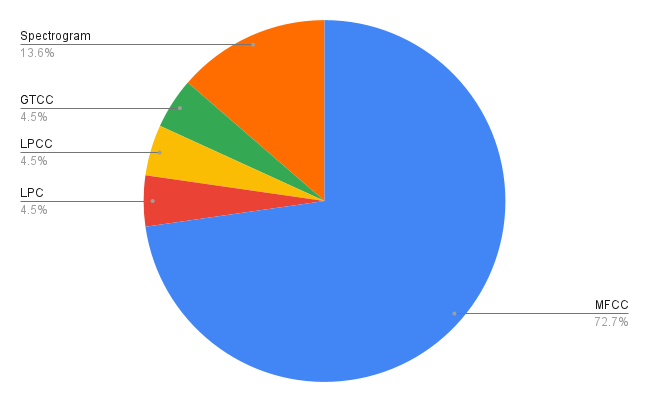
\includegraphics[scale=0.50]{lit_review_images/chartFeatureExtraction.png}
    \caption{A chart showing the frequency of methods used to detect/extract emotional features from audio.}
    \label{figure:featureExtractionUsage}
\end{figure}

Notably, the use of tools such as openSMILE toolkit by audEERING is observed in several studies. OpenSMILE is a feature extractor that can be configured to extract specific features from audio and music signals for signal processing and machine learning, emphasising features enabling emotion recognition from speech. The paper by \cite{Anjum2019-ks} decided to test several of the extractable features for their application in emotion recognition, they tested: Intensity, Loudness, 12 MFCC, Pitch (f0), Probability of Voicing, F0 Envelope, 8 LSF and Zero-Crossing Rate. Once collected, they select the best features with a `BestFirst' approach.  These features were then classified, testing 3 different classification methods: multilayer perceptron neural networks, Rules Classifier oneR, and Tree Classifier J48. Their results showed that the multilayer Perceptron neural network had the best performance. A couple of other methods utilising this feature extraction method employed different networks for their classification, one choosing a Two-Layer Fuzzy Random Forest ensemble classifier \cite{Chen2020-bt}, and another a SVM \cite{Ashok2022-xp}.

Attention-based speech emotion recognition models have garnered significant attention in recent years due to their ability to capture relevant features from audio data effectively, thus improving the precision of emotion classification tasks \cite{Peng2020-wv}. By dynamically weighting different segments of the input speech signal \cite{Zhichao2020-bf} based on their importance in expressing emotional content, these models offer a promising approach to discern subtle nuances in speech patterns associated with various emotional states \cite{Nie2022-fo}. Using mechanisms inspired by human attentional processes, such as self-attention and multi-head attention \cite{Rasendrasoa2022-nf}, these models excel in identifying salient acoustic cues indicative of specific emotions, thus paving the way for more nuanced and contextually rich emotion recognition systems.

\subsection{Applications}

In a study on speech emotion recognition in speaker-independent systems, specifically for the Mung robot \cite{Kim2009-in}, two key strategies were proposed to improve accuracy and reliability. The first strategy involves separating emotion recognition from consonants and obstruents to reduce text dependency and enhance adaptability. The second strategy introduces a rejection algorithm based on a confidence measure to ensure more reliable outcomes. Comparative analysis with conventional methods showed significant improvements, with recognition rates increasing from 6.9\% to 27.6\% across various emotional features through the separation algorithm and 73\% to 92\% with the confidence-based rejection mechanism for MFCCs \cite{Kim2018-dh}.

In a paper by Carolis, B.D. \cite{Carolis2016-ig}, they use the Nao robot combined with a module that they developed called the VOCE 2.0. A module designed to classify speech used to send requests by features extracted according to dimensional models, valence, and arousal. They encountered low performance; however, they attribute this to the training data, the \begin{math}\in{}\end{math}motion dataset, and their target audience of elderly individuals, which have a different range of characteristics.

Research has highlighted the indispensable role of data augmentation techniques in strengthening speech-emotion recognition systems. Lakomkin et al.\ \cite{Lakomkin2018-ws} carried out a study to evaluate the impact of data augmentation by testing two models, one with data augmentation and the other without. Their analysis, especially when using the iCub robot as a test bed, demonstrated a significant drop in overall resilience and effectiveness for the model that did not incorporate data augmentation. These results serve as a compelling reminder of the critical importance of utilising data augmentation strategies to improve the performance of speech-emotion recognition systems.

\section{Gesture-based Emotion Recognition}

Gesture-based emotion recognition focuses on interpreting emotional states from non-verbal body cues such as posture, movement, and hand gestures. These cues play a critical role in affective communication, particularly in scenarios where facial expressions or speech are unavailable or unreliable, such as when a person is wearing a mask, facing away, or in silence.

This section reviews both the algorithmic approaches used to extract and classify emotional information from gestures, as well as practical applications in interactive robotic settings.

\subsection{Datasets}

The Body Emotion Expression (BEE) dataset \cite{Elfaramawy2017-ab} captures six emotions, anger, fear, happiness, neutral, sadness, and surprise, from 19 participants with diverse cultural backgrounds. Using two Nao robots, one equipped with a depth sensor, body motions were recorded from frontal and side views. Participants performed both neutral and emotionally driven actions inspired by brief scenarios. The dataset includes 570 sequences, with 3D skeleton data extracted from 11 key body joints.

The H80kPartial dataset \cite{8578328} is a subset of the larger H80k (Humans 80k) dataset, specifically designed for emotion recognition through human pose analysis. This dataset focuses on capturing human body postures and gestures that are indicative of emotional states. It contains annotated data that emphasise partial body poses, such as the upper body, arms, and facial orientation, to help identify emotional expressions without requiring full-body information.

\subsection{Algorithms}

The analysis of human gestures to understand emotional states is a crucial aspect of affective human-human interaction. Body movements, hand gestures, and facial expressions are among the non-verbal cues that provide valuable emotional information. In situations where verbal or facial cues are limited, such as when someone is wearing a face mask, gesture-based emotion recognition is essential, leading to more intuitive and empathetic interactions between humans and machines.

Marinoiu et al.\ \cite{8578328} explore the complexities of recognising emotions through gestures, focusing on adapting state-of-the-art RGB 3D human pose reconstruction methods that blend feedforward and feedback components. Their study compares several baselines for recognising actions and emotions using 2D and 3D representations of both children and therapists. The results suggest that with proper adaptation, current RGB-based 2D and 3D reconstruction methods can rival industrial-grade RGB-D Kinect systems. They employed methods like DMHS (Deep Multitask Architecture for Integrated 2D and 3D Human Sensing) and a custom variant, DMHSPV, to extract features and introduced a new dataset, H80kPartial. While CNNs outperformed RNNs in emotion recognition, their findings highlight the ongoing efforts to enhance gesture-based emotion recognition.

Wang et al.\ \cite{Wang2022-eq} have introduced an innovative method for touch gesture and emotion recognition called Multi-Task Touch Gesture and Emotion Recognition (MUSCAT). This approach involves using a fabric embedded with touch sensors that mimic human skin, allowing accurate touch gesture recognition. The results of the TouchGET and CoST datasets demonstrate that the MUSCAT method significantly reduces computation costs while improving classification accuracy. Furthermore, the incorporation of Multi-Task Learning (MTL) further enhances classification performance, validating the effectiveness of the proposed MUSCAT method and MTL framework in touch gesture and emotion recognition.

Lyu and Sun \cite{Lyu2022-vd} faced a unique challenge in the field of dance emotion recognition for robots, which presents numerous difficulties because video-based emotion detection is vulnerable to various external factors. To overcome these obstacles, the authors created a strong multi-feature fusion framework that combines global and local features using an LSTM mechanism. The study used three distinct data sets: RML, SAVEE, and a self-constructed dance video database. The experimental process involved training and testing on these datasets, which produced promising results that demonstrated the effectiveness of their proposed feature extraction algorithm. Notably, their approach surpassed single-feature methods, showing the viability of emotion recognition from dance.

The integration of multimodal sensory information presents a critical challenge in the development of advanced human-machine affective systems. A research article titled `Deep Emotion Recognition through Upper Body Movements and Facial Expression' by Aqdus et al.\ \cite{Aqdus2021-xr} delves into this challenge, focusing on spatial-temporal techniques for emotion analysis across visual modalities.

The study explores the fusion of two primary modalities: facial expressions and upper-body movements. The researchers aimed to develop a robust architecture capable of identifying emotions in real-time human-machine interaction systems. Their findings highlight the superiority of the bimodal approach over those of monomodal ones, regardless of the fusion method applied. In particular, the study achieved the best recognition rates for anger, happiness, and neutral emotions, while the worst recognition rate was observed for sadness, often misclassified as surprise. Evaluation metrics consistently demonstrated significant improvements in accuracy, moving from 77.7\% and 76.8\% for the recognition of emotion from facial and upper body movements, respectively, to 85.7\% and 86.6\% after the fusion of both modalities.

While effective in experimental settings, these methods often require a fixed camera and precise calibration, making them difficult to scale or adapt to a robot intended to move around.

\subsection{Applications}
Marinoiu et al.\ \cite{8578328} present a gesture-based emotion recognition approach with strong implications for robot-assisted therapy, particularly in recognizing emotions expressed by children and therapists. Their system enables non-invasive emotional monitoring in developmental contexts such as autism therapy. The researchers employ the Zeno robot, a humanoid platform specifically designed to support children with autism. By recognizing emotions through gestures and body movements, Zeno enhances its interactive capabilities, making it a promising tool for empathetic and adaptive therapeutic interventions.

Elfaramawy et al.\ \cite{Elfaramawy2017-ab} apply their gesture-based emotion recognition framework in a HRI setting involving two Nao humanoid robots. One Nao is equipped with an Asus Xtion depth sensor, positioned to capture depth-map video sequences from multiple angles, while the second robot facilitates interaction from a side perspective. This setup enables the collection of frontal, side, and rear views of participants as they express emotions through full-body movement. To elicit spontaneous emotional behavior, participants were prompted with realistic roleplay scenarios (e.g., for fear, imagining a break-in and requesting the robot to call for help). This experimental design yielded a rich, multi-view dataset of emotional body expressions.

\section{Multi-modal Emotion Recognition}

Multi-modal emotion recognition systems combine various data sources, such as visual, auditory, and gesture signals, to enhance the accuracy and robustness of emotion detection. By integrating multiple modalities, these systems can capture a more comprehensive understanding of human emotions, aiming to improve performance in real-world applications. This section reviews the datasets and algorithms used in multi-modal emotion recognition, highlighting their significance in advancing the field.

\subsection{Datasets}

The FABO (FAcial and BOdily Expression) dataset \cite{1699093} plays a significant role in multimodal emotion recognition, as it captures both facial expressions and body postures across a range of emotions. With recordings from 23 subjects displaying ten different emotional states, the dataset emphasises the importance of bodily cues in recognising emotions. This makes FABO particularly valuable for research focused on pose-based emotion recognition, where body language and movement are key to identifying emotions. The combination of facial and bodily data allows for a more comprehensive analysis of how emotions are expressed physically, supporting the development of robust, multimodal recognition systems.

\subsection{Algorithms}

Multimodal emotion recognition systems aim to improve the accuracy and reliability of emotion detection by incorporating multiple types of input data, such as visual, auditory, physiological, or textual information. By drawing from diverse sources, these systems can capture a more comprehensive understanding of human emotions. Some approaches integrate these modalities into a unified output, combining the strengths of each to enhance overall performance. Others treat each modality independently, using one to validate or back up the other in cases of ambiguity or failure. The fusion of modalities allows for more robust emotion recognition, particularly in complex, real-world settings where single modalities may fall short.

Studies such as \cite{Song2018-vu} have investigated classification techniques for combining various modalities, artificial neural networks (ANN) with k-nearest neighbours (k-NN). Decision trees were also employed by \cite{Adiga2020-wv} having a simple CNN for facial detection and a log-Mel spectrum for feature extraction from speech.

Kansizoglou et al.\ \cite{Kansizoglou2022-ih} used two CNNs, one for audio recognition and one for facial expression recognition, together with a DNN to fuse them; a long- and short-term memory (LSTM) layer and a Reinforcement Learning (RL) agent are trained in cascade, stopping feature extraction for final prediction. Additionally, using a Haar cascade for initial face cropping, they employ MobileNetV2 for image classification and a VGG architecture for audio, both retrained on emotion recognition datasets. The results indicate improved accuracy through fusion, albeit with some emotion confusion, tested on RML and BAUM-1 datasets.

In the pursuit of advancing multimodal emotion recognition within the realm of HRI, Yu and Tapus \cite{Yu2019-ku} present a study titled `Interactive Robot Learning for Multimodal Emotion Recognition.' Their research employs a sophisticated experimental setup featuring a Kinect and an Optris thermal camera to capture human gait information and thermal facial images for emotion recognition. This study developed a multimodal emotion recognition model grounded in gait and thermal facial data, using a random forest (RF) model and modified confusion matrices of two individual models. A comparative analysis between individual RF models and the hybrid decision-level model demonstrates the effectiveness of their integration method in classifying emotions during HRI. Moreover, the extensive experimentation involving online testing before and after Interactive Robot Learning (IRL) substantiates that interactive robot learning is a valuable technique, yielding a significant increase of more than 10\% in the accuracy of multimodal emotion recognition with gait and thermal data. Yu and Tapus \cite{Yu2020-zq} even attempted to further improve upon their innovative thermal imaging plus human gait information for emotion recognition by implementing WaveNet to get more benefits from spatial and temporal information.

Chen et al.\ \cite{Chen2023-ss} have introduced a groundbreaking approach to multimodal emotion recognition in HRI called Coupled Multimodal Emotional Feature Analysis (CMEFA). This method utilises a Broad-Deep Fusion Network (BDFN) to extract emotional features from facial expressions and gestures. By applying Canonical Correlation Analysis (CCA) to capture the correlation between these features, CMEFA offers a more comprehensive understanding of emotional cues. A coupling network recognises emotions based on the extracted bi-modal features. Remarkably, simulation experiments conducted on the FABO database demonstrate the superiority of CMEFA over existing methods, outperforming the SVM Recursive Feature Elimination (SVMRFE) method by achieving a recognition rate of 1.15\% higher and exceeding other approaches by significant margins.

In addition, the researchers conducted preliminary application experiments on an emotional social robot system, where the robot successfully recognised emotions based on the facial expressions and body gestures of the volunteers. This showcases the practical applicability of CMEFA in real-world scenarios.

Several studies have emerged focusing on sentiment analysis, addressing this gap in research. For example, Augello et al.\ \cite{Augello2022-zy} presented `Multimodal Mood Recognition for Assistive Scenarios' showcasing the effectiveness of their approach in detecting emotions from textual data. Additionally, Heredia et al.\ \cite{Heredia2022-dt} proposed the `Adaptive Multimodal Emotion Detection Architecture for Social Robots,' incorporating natural language processing (NLP) transformers and an emotion ontology to enhance emotion detection capabilities in social robots. Sentiment analysis shows promise in working in a resource constrained environment, this can also be offloaded to a cloud service, allowing for more complex models to be used without the need for high computational power on the robot itself.

Temporal features have emerged as a significant benefit for multimodal emotion recognition systems. Research efforts such as those by Hung et al.\ \cite{Hung2020-gm} have focused on leveraging temporal feature learning to improve emotion recognition accuracy, highlighting the effectiveness of using multiple models to capture temporal dynamics in emotional expressions.

\subsection{Applications}

While multimodal emotion recognition has advanced rapidly in theory, its deployment on robotic platforms remains sparse. Practical constraints, such as real-time processing, hardware limitations, and environmental variability, have limited its adoption. However, emerging applications show promise in enriching robot perception and interaction.

In one of the few real-world implementations of multimodal emotion recognition on a robotic platform, Yu and Tapus \cite{Yu2019-ku} employed the Pepper robot in a controlled laboratory setting. Their system combined thermal facial imaging, captured via an Optris thermal camera, with gait analysis using a Kinect sensor, allowing the robot to infer emotional states from both body movement and facial temperature cues. The experimental procedure involved 8 participants, each completing 24 sessions across three phases: initial online testing, an intermediate interactive robot learning (IRL) phase, and post-IRL testing. A total of 192 sessions were conducted over the course of one month. Environmental variables such as lighting and temperature were tightly controlled to ensure data consistency.

Another real-world deployment of multimodal emotion recognition in robotics was demonstrated in a preliminary application experiment involving an emotional social robot system. The setup utilized a Kinect sensor to capture full-body and facial data under natural indoor lighting conditions, enabling emotion inference based on both posture and facial expressions. Eight postgraduate participants (balanced by gender) were recruited to express the seven basic emotions, with peak emotional states used for training. During testing, an emotion was considered correctly recognized if the system identified the apex state accurately. The experiment achieved an average recognition accuracy of 75.85\%. While misclassifications were largely attributed to environmental factors and limitations in the face and body detection algorithms, the results highlight the feasibility and promise of deploying multimodal emotion recognition in affective HRI scenarios \cite{Chen2023-ss}.

\section{Table Of Robots}
The following table provides a consolidated overview of robotic platforms used in emotion recognition and HRI research. For each robot, the table includes its name, a representative image, and references to studies detailing its application or implementation. References are annotated according to the modalities employed in each study. This compilation illustrates the diversity of robots explored in the literature, highlighting their distinct capabilities and roles in enabling emotionally aware and socially responsive interactions with humans.
% Table of Robots
\begin{table}[h]
\centering{}
\caption{Table of all Robots in Literature}
\hspace*{-1in}
\resizebox{\linewidth+3cm}{!}{
\begin{tabularx}{1.3\textwidth}{ c|X|X|c|c|}
\cline{2-5}
\textbf{} & \textbf{Robot Name} & \textbf{Facial} & \textbf{Audio} & \textbf{Gesture}\\
\cline{2-5}
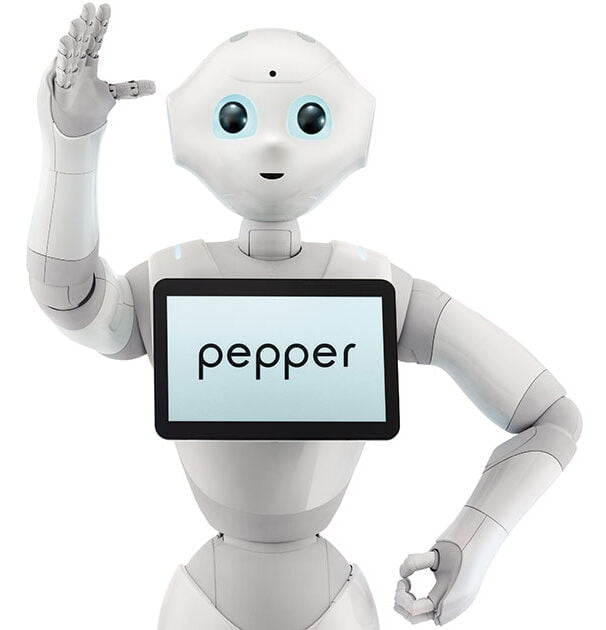
\includegraphics[width=0.15\textwidth]{robot_table/pepper.jpg} & Pepper  & \cite{Yu2019-ku} \cite{Yu2020-zq} & & \cite{Yu2019-ku} \cite{Yu2020-zq}  \\
\cline{2-5}
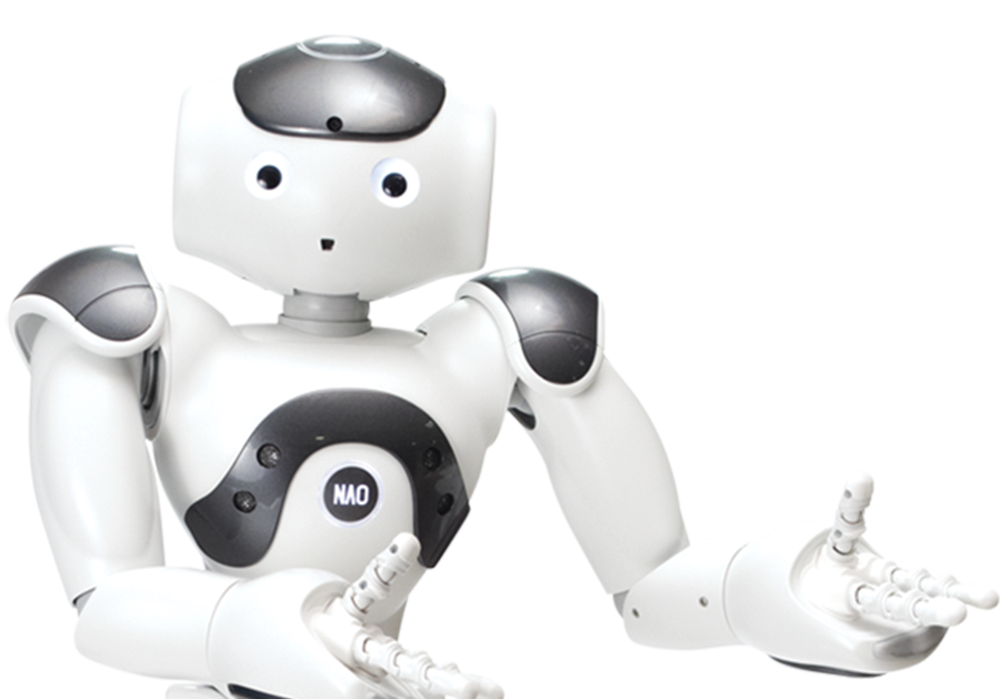
\includegraphics[width=0.2\textwidth]{robot_table/Nao.png} & Nao     & \cite{Faria2017-lg} \cite{10.1007/s11042-022-12794-3} \cite{Lopez-Rincon2019-et} \cite{Melinte2020-ky} \cite{Rosula_Reyes2020-yz} \cite{Ruiz-Garcia2018-zq} \cite{Ruiz-Garcia2018-uy} \cite{9900581} \cite{Webb2020-bq} \cite{10008155} & \cite{Carolis2016-ig} & \cite{10008155} \\
\cline{2-5}
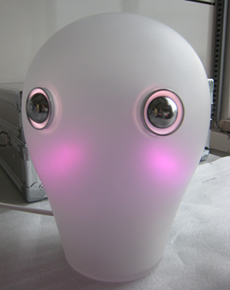
\includegraphics[width=0.12\textwidth]{robot_table/Mung_001.jpg} & Mung    & & \cite{Kim2018-dh}  & \\
\cline{2-5}
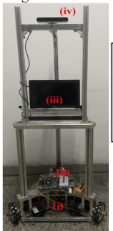
\includegraphics[width=0.08\textwidth]{robot_table/ODSR.png} & Omnidirectional Service Robot & \cite{9982640}  & \cite{9982640} & \\
\cline{2-5}
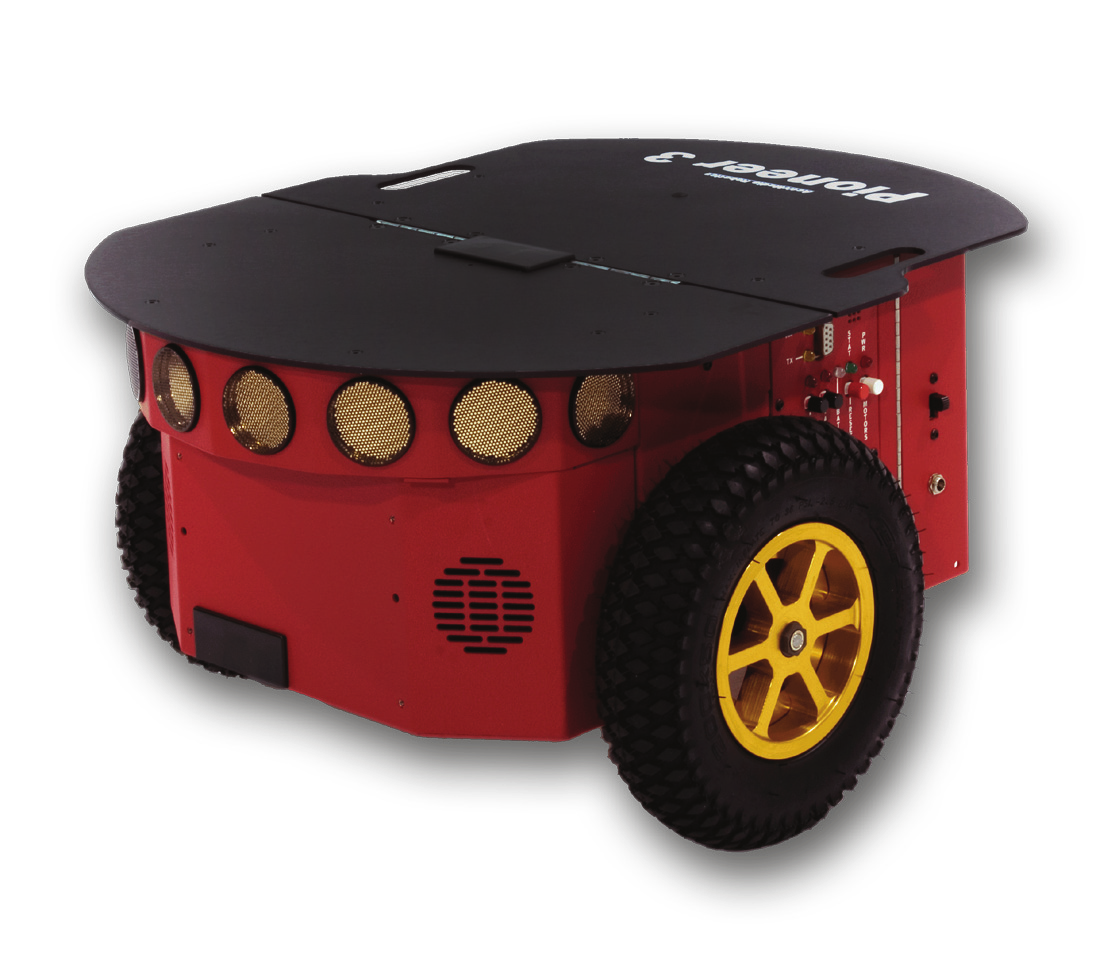
\includegraphics[width=0.2\textwidth]{robot_table/pioneer3dx.png} & Pioneer P3-DX robot, LARa robot  & \cite{8588580}  & \cite{8588580} & \\
\cline{2-5}
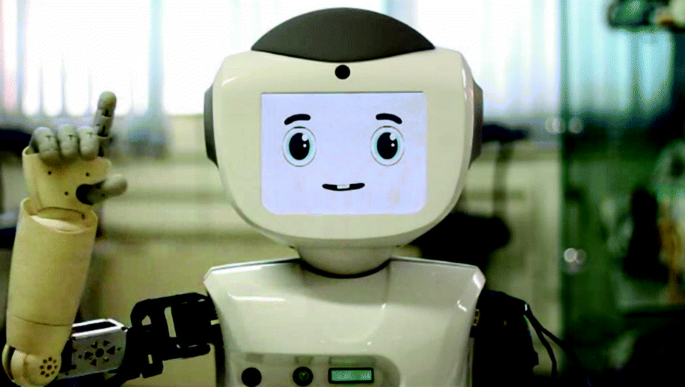
\includegraphics[width=0.2\textwidth]{robot_table/RASA.png} & RASA    &  & \cite{Esfandbod2023-eq} & \\
\cline{2-5}

\includegraphics[width=0.11\textwidth]{robot_table/ohmni.jpg} & Ohmni & \cite{Devaram2022-qc}  & & \\
\cline{2-5}
\end{tabularx}
}
\end{table}
\clearpage{}

\begin{table}[ht]
\centering{}
\caption{Table of all Robots in Literature Cont.}
\hspace*{-1in}
\resizebox{\linewidth+3cm}{!}{ % Extend beyond text width
\begin{tabularx}{1.3\textwidth}{ c|X|X|c|c|}
\cline{2-5}
\textbf{} & \textbf{Robot Name} & \textbf{Facial} & \textbf{Audio} & \textbf{Gesture}\\
\cline{2-5}

\includegraphics[width=0.2\textwidth]{robot_table/iCub.jpg} & iCub    & & \cite{Lakomkin2018-ws} &  \\
\cline{2-5}

\includegraphics[width=0.12\textwidth]{robot_table/ROBIN.png} & ROBIN   & & \cite{Ashok2022-xp} &  \\
\cline{2-5}
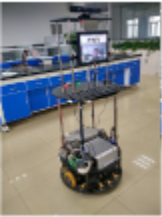
\includegraphics[width=0.2\textwidth]{robot_table/ESRS.png} & ESRS (Emotional Service Robot System) & \cite{CHEN202010236} \cite{Chen2021-ra} \cite{CHEN201849}  & &   \\
\cline{2-5}
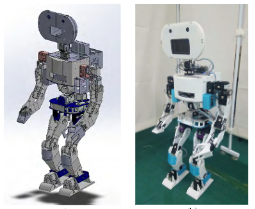
\includegraphics[width=0.2\textwidth]{robot_table/Harley.png} & Harley  & \cite{8760246}  & &  \\
\cline{2-5}
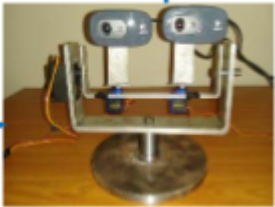
\includegraphics[width=0.2\textwidth]{robot_table/RobotEye.png} & Robot eye & \cite{Appuhamy2018-dc}  & &  \\
\cline{2-5}
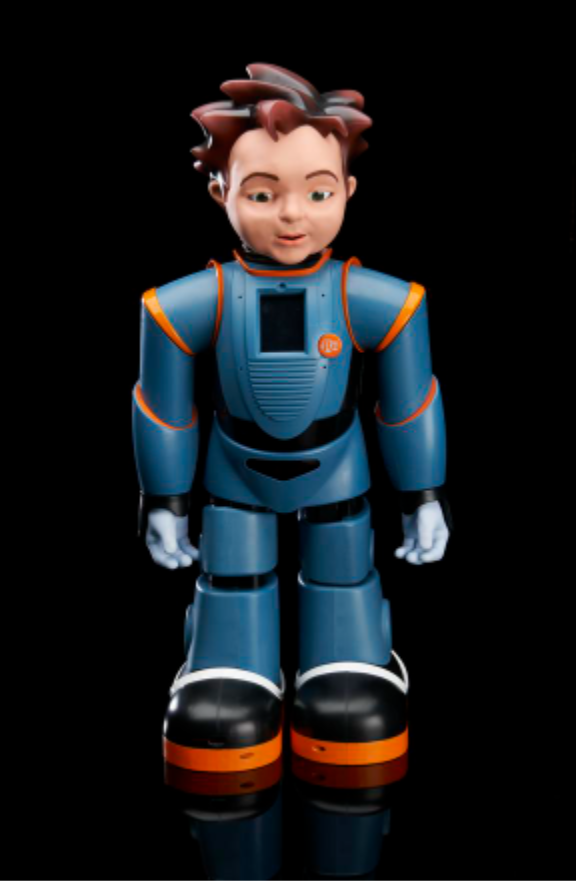
\includegraphics[width=0.2\textwidth]{robot_table/Zeno.png} & Zeno    & & & \cite{8578328}  \\
\cline{2-5}
\end{tabularx}
}
\end{table}
\clearpage{}

\section{Critical Review of Invasive Technology for Emotion Recognition}
Emotion recognition technologies have made significant advances in recent years, with various invasive and less invasive techniques being developed to better capture emotional states. These technologies can be broadly categorised into electro-based systems, physiological sensors, and non-contact methods. Although each approach has its strengths, they also present notable limitations, particularly in terms of user comfort and practicality for real-world application. This review critically evaluates key technologies for emotion recognition, outlining their mechanisms, benefits, and drawbacks.

\subsection{Electro-Based Technologies}
Electro-based methods such as EEG (Electroencephalography), EMG (Electromyography), EOG (Electrooculography) and ECG (Electrocardiography) are commonly used in emotion recognition due to their ability to capture direct biosignals from the brain and body. EEG, for example, measures brain electrical activity and is used to classify emotional states based on asymmetries in the prefrontal cortex. High arousal emotions (e.g., joy, anger) are associated with greater activity of the left frontal cortex, whereas low arousal emotions (e.g., fear, sadness) show increased activity of the right frontal \cite{Suhaila2021-dh}. However, EEG signals vary significantly between individuals, making the development of universal models challenging \cite{Pal2021-eq}. Furthermore, EEG setups require sensors attached to the scalp, which limits practicality in nonlaboratory settings due to discomfort and susceptibility to movement artefacts, particularly head movements \cite{Tan2021-ai}.

EMG, on the other hand, measures muscle activity and is used to detect emotional expressions through facial or bodily muscle movements. For example, negative emotions correlate with high activity in the corrugator supercilii (frowning muscles), while positive emotions exhibit reduced activity in this region \cite{Suhaila2021-dh}. Although it is an effective tool for detecting nuanced emotional expressions, EMG requires that sensors be placed directly on the skin, which can be intrusive and uncomfortable, especially in dynamic everyday situations.

The electrocardiogram (ECG) is another key method, used to measure the electrical activity of the heart, enabling the detection of emotional reactions by analysing the variability of heart rate (HRV). Similar problems arise with EOG, which tracks eye movement and pupil dilation, but again requires physical contact with sensors around the eyes \cite{Dzedzickis2020-hf}.

Overall, these electro-based systems excel in providing high-quality, detailed emotion-related data, yet their invasive nature and reliance on stationary or controlled environments impede their adoption in daily life. In terms of precision, multimodal recognition systems, such as those that combine EEG and facial expression recognition through convolutional neural networks (CNNs), have been shown to perform better. For example, integrating EEG signals and facial data through plurality voting classifiers and the Monte Carlo method achieved an impressive accuracy of 83.33\% \cite{Tan2021-ai}.

\subsection{Physiological Sensors}
Recent developments in physiological sensors aim to reduce invasiveness while still collecting valuable emotion-related data. Devices such as the Microsoft Band 2 and smartphones use less invasive sensors to monitor heart rate, skin temperature, and galvanic skin response (GSR) through optical heart rate monitors, accelerometers, and UV sensors. These sensors are more practical for daily use, as they are worn externally and do not require direct contact with the skin in multiple locations \cite{Younis2022-bs}.

For example, GSR measures skin conductivity and can indicate emotional arousal, with increased conductance correlated with emotional intensity. Skin temperature sensors also provide information on emotional states, as temperature tends to increase during negative emotions such as anger and decrease during positive emotions such as calm \cite{Nawasalkar2017-fx}. Furthermore, heart rate and breathing rate can be monitored non-invasively, with quicker, deeper breaths often associated with negative emotions and slower breaths with positive emotions \cite{Younis2022-bs}. 

Although these less invasive devices offer improved user comfort, they are limited in their ability to capture precise emotional nuances, often requiring advanced signal processing and analysis algorithms to compensate for lower signal-to-noise ratios. For example, remote photoplethysmography (rPPG) enables heart rate monitoring without direct skin contact by analysing light reflected from the skin. Although it increases user comfort, the reduced accuracy due to environmental factors such as lighting conditions and motion noise presents a challenge \cite{Dzedzickis2020-hf}.

Similarly, a Doppler radar-based system, used to track chest movements to extract heart rate and breathing patterns, offers non-contact emotion recognition. However, this technology is more suitable for controlled environments, as everyday movements can distort signals \cite{Lubecke-4751478}.

\subsection{Challenges of Invasive Emotion Recognition}
The most significant challenge with invasive emotion recognition technologies is the discomfort and practicality issues associated with attaching sensors to the skin or body. The use of contact-based systems, such as EEG, ECG, EOG, and EMG, creates limitations for their use in real-world applications where people need to move around, introducing noise. These technologies excel in laboratory environments where user movements can be controlled and minimised. 

In addition to comfort, generalisability remains a concern. EEG signals, for example, are subject-dependent, meaning that models developed for one person may not be easily transferable to others. This limits the scalability of EEG-based systems for broader applications, particularly in healthcare or consumer devices.

Invasive emotion recognition technologies, while highly effective in controlled environments, face significant barriers to widespread adoption in real-world scenarios. Electro-based methods like EEG and ECG provide detailed biosignals for emotion classification, but their need for skin contact and susceptibility to movement interference limits their practicality. Less invasive approaches, such as physiological sensors and non-contact methods such as rPPG and Doppler radar, offer greater user comfort but often sacrifice signal quality, requiring more advanced processing techniques to maintain accuracy.

\section{Discussion}
While current multimodal emotion recognition systems exhibit promising capabilities, several gaps remain that could enhance their performance and applicability in real-world scenarios. One notable gap is the reliance on Haar Cascade for facial detection across various papers. Although Haar Cascade has been a staple in face detection due to its simplicity and efficiency, it may not offer the highest recognition rates compared to more advanced techniques. Models such as YOLO (You Only Look Once) \cite{Redmon2015-eb}, or HOG+Linear SVM \cite{Singh2020-ui} could provide superior accuracy and robustness in detecting faces in diverse conditions. By exploring these alternative models, it is plausible that the subsequent emotion recognition processes will also improve, ultimately leading to more effective HRIs.

Furthermore, the integration of cloud-based tools presents a significant opportunity to enhance multimodal emotion recognition systems. Current approaches utilising sentiment analysis do not fully leverage the potential of cloud computing, which can significantly offload processing tasks from local systems. By moving computationally intensive operations to the cloud, valuable resources can be freed up for other essential tasks, such as real-time interaction and response generation. Such an architecture could enhance the scalability and flexibility of emotion recognition systems, enabling them to adapt more readily to varied user interactions and environmental contexts.

By addressing these gaps, this research intends to develop a more sophisticated emotion recognition system capable of accurately interpreting human emotions in a wider range of scenarios. The continued exploration of advanced face detection techniques and the adoption of cloud-based solutions could lead to significant advancements in the reliability and effectiveness of multimodal emotion recognition, ultimately enhancing the capabilities of robotic systems in understanding and responding to human emotional states.


